\documentclass[11pt, twoside]{report}
\usepackage[utf8]{inputenc}
\usepackage{graphicx}
\usepackage{wrapfig}
\usepackage[a4paper, width=150mm, top=25mm, bottom=30mm, bindingoffset=20mm]{geometry}
\usepackage[toc,page]{appendix}
\usepackage{pdfpages}
\usepackage{natbib}
\usepackage{pdflscape}
\usepackage{longtable}
\usepackage{tikz}
\usepackage{multirow}
\usepackage{textcomp}
\usepackage{fancyhdr}
\usepackage{helvet}
\usepackage{hyphenat}
\usepackage{listings}
\usepackage{color}	
\usepackage[hidelinks]{hyperref}
\usepackage{pgfplots}
\usepackage{subcaption}
\usepackage{array}
\usepackage{longtable}
\usepackage{enumitem}
\usepackage[export]{adjustbox}
\usepackage{lscape}
\usepackage{titlesec}
\usepackage{tabularx}
\usepackage{booktabs}
\newcolumntype{L}[1]{>{\raggedright\let\newline\\\arraybackslash\hspace{0pt}}m{#1}}
\newcolumntype{C}[1]{>{\centering\let\newline\\\arraybackslash\hspace{0pt}}m{#1}}
\newcolumntype{R}[1]{>{\raggedleft\let\newline\\\arraybackslash\hspace{0pt}}m{#1}}
\renewcommand{\familydefault}{\sfdefault}
\def\checkmark{\tikz\fill[scale=0.4](0,.35) -- (.25,0) -- (1,.7) -- (.25,.15) -- cycle;} 
\pagestyle{fancy}
\fancyhf{}
\fancyhead[LE, RO]{\thepage}
\fancyhead[LO, RE]{\leftmark}
\fancyfoot[c]{Bournemouth University, Department of Computing and Informatics, Final Year Project}
\setlength{\headheight}{13.6pt}
\linespread{1.3}
\bibliographystyle{buHarvard}
\bibpunct{(}{)}{,}{a}{}{ }
\graphicspath{ {images/}{appendices/} }
\footskip = 15mm
\definecolor{mygreen}{rgb}{0,0.6,0}
\definecolor{mygray}{rgb}{0.5,0.5,0.5}
\definecolor{mymauve}{rgb}{0.58,0,0.82}
\pgfplotsset{compat=1.13}

\lstset{ %
  backgroundcolor=\color{white},   % choose the background color; you must add \usepackage{color} or \usepackage{xcolor}
  basicstyle=\ttfamily\footnotesize,        % the size of the fonts that are used for the code
  breakatwhitespace=false,         % sets if automatic breaks should only happen at whitespace
  breaklines=true,                 % sets automatic line breaking
  captionpos=b,                    % sets the caption-position to bottom
  commentstyle=\color{mygreen},    % comment style
  escapeinside={\%*}{*)},          % if you want to add LaTeX within your code
  extendedchars=true,              % lets you use non-ASCII characters; for 8-bits encodings only, does not work with UTF-8
  keepspaces=true,                 % keeps spaces in text, useful for keeping indentation of code (possibly needs columns=flexible)
  keywordstyle=\color{blue},       % keyword style
  otherkeywords={*,...},           % if you want to add more keywords to the set
  numbers=left,                    % where to put the line-numbers; possible values are (none, left, right)
  numbersep=5pt,                   % how far the line-numbers are from the code
  numberstyle=\tiny\color{mygray}, % the style that is used for the line-numbers
  rulecolor=\color{black},         % if not set, the frame-color may be changed on line-breaks within not-black text (e.g. comments (green here))
  showspaces=false,                % show spaces everywhere adding particular underscores; it overrides 'showstringspaces'
  showstringspaces=false,          % underline spaces within strings only
  showtabs=false,                  % show tabs within strings adding particular underscores
  stepnumber=1,                    % the step between two line-numbers. If it's 1, each line will be numbered
  stringstyle=\color{mymauve},     % string literal style
  tabsize=2,	                   % sets default tabsize to 2 spaces
}


\begin{document}
\pagenumbering{Alph}

%TC:ignore

\includepdf{cover.pdf}
\pagenumbering{roman}

\vspace*{\fill}
\begingroup
\centering
Faculty of Science \& Technology

Department of Computing and Informatics

Final Year Project

\endgroup
\vspace*{\fill}

%!TEX root = ../main.tex
\chapter*{Abstract}
It can be difficult for parents to motivate children to perform given chores or tasks in a timely manner.
This project aims to create a system for parents to help encourage children in the form of a gamified task management mobile app.
The app will reward children for performing a task using a popular video game based reward structure by offering `Experience Points', which will, when collected, allow them to level up their character.  
This report will detail how I have designed and developed the system surrounding these goals.

Research will be performed into the study of motivation and rewards, particularly with children, and into what will be the best tools I can implement to benefit this.

The artefact has been created as a central server based REST API that receives and handles web service requests to return JSON data.
This API is interfaced via an Android application which will display the received data in an aesthetically pleasing and informative format.

I have approached this project using agile and test driven development methodologies to create a well structured and reliable software artefact.
Requirements were gathered using brainstorming skills and were refined using the MoSCoW method to create a list of features that I believed would motivate children to perform tasks.

\input{chapters/bustuff}

%!TEX root = ../main.tex
\chapter*{Acknowledgements}
These are my acknowledgements

%Lys
%Damien
%Jake
%The good people of StackOverflow

\hypersetup{
	citecolor=black,
	filecolor=black,
	linkcolor=black,
	urlcolor=black
}

\tableofcontents
\listoffigures

\cleardoublepage
\pagenumbering{arabic}

%TC:endignore

%1000 words
%!TEX root = ../main.tex
% What is the project about? 
% What problem are you tackling? 
% What is your research question? 
% Why do these problems need solutions? Why are they important?
% What is the background to the problem? Who is the client? What do they want?
% What existing methods have been tried? How has I.T. been applied so far? 
% What constraints do you have? (Time, PCs, money, users, software etc) 
% What is the scope of what you have set yourself to do. What is not included?
% What broad approach was taken? (Summarise your broad approach the project) 
% Risk management summary

% 1000-2000 words

\chapter{Introduction}
\label{chap:intro}

\section{Problem Definition}
Parents often find it difficult to motivate children to perform chores in a timely manner. 
Many parents have attempted to implement a simple reward system to incentivize their children, but often fail to keep up with the rewards or maintain the tracking  

\section{Aims and Objectives}

\section{Proposed Artefact}
I want to create a mobile application that will allow parents to assign tasks and rewards to their children in the form of ``quests'' in a role-playing game, effectively gamifying chores. 
The quests can take the form of “Tidy your room” or “Complete your homework” and offer rewards of experience points and gold to level up the child's in-game avatar. 
I believe the app will provide children with incentive and positive reinforcement to acheive more.

Inspiration from this project came from two main sources: Habitica (Previously: HabitRPG), which sought to help people better themselves by adding their own tasks and to-do lists as quests and completing them to earn self-defined rewards. 
However, this game focuses largely on the self-improvement of adults and required people to self manage the software, whereas KidQuest will provide the separation of adult and child to help parents motivate their children.

Secondly, an experiment at Indiana University, where a professor chose to give out XP rewards and levels instead of letter based grades \cite{sheldon2011multiplayer} 

The key clients for this app will be the parent(s) inputting quests into the game and marking a quest as complete once they have inspected the work. 
The child will also be able to view quests, notify the parents that a quest requirement is ready for inspection and choose skills and equipment for their character. 
Whilst parents will be able to monitor their children's activities and progress, whilst approving or rejecting various interactions that the child may have on the app.

\section{Risks}
As this is a solo development project, there is a significant risk that there will be flaws in the initial design. 
This is due to the fact - coupled with the fact that this is new technology to me - that there is a high probability that I will misunderstand what is needed for certain designs or misunderstand what the correct tool for the job is.
Because of this I would argue that during this project, it is almost certain that the initial spec for this project will change and redesigns will need to be made. 
In order to mitigate this, I have taken steps to make individual features and sections of the code of the project as modular as possible, hoping to be able to swap out sections of the code should certain changes arise.
I will also code many aspects of the app with the idea that it may move to a server back-end, rather than having data stored in the app. 
 
The risk of changes in turn raises a key risk to the project which is that it may not be ready for the deadline. 
I consider this to be a high severity risk to the project, as the hand-in date for the project is firm and unchangeable. 

As I am the only developer on the project, there is a high risk of the code quality being lower than what can be expected from a team.
I am undertaking a self code-review policy, where I reserve some time to inspect the code of each feature branch before it is merged into the master branch.
I believe that if I am sufficiently strict with the reviews, they will help me ensure that code quality is kept up to an acceptable standard.
Arrangements have also been made with a fellow course member to code review each others code as our projects are sufficiently different enough to avoid plagiarism and we both have strong interests in keeping our code quality to a high standard.
When utilized correctly, code review can find approximately 30-70\% of logic errors within a program \citep{myers2011art}.

Another risk that may arise is the potential for hardware failure. 
Should it occur, it could wipe out the codebase and the project report, effectively destroying the project. 
Whilst it is unlikely, steps must still be taken to mitigate this, and so I will store both the code and the report in multiple local and remote locations.
The report, app code and server code will all be stored on both my PC and my Laptop as a local backup, and all three will also be stored in a remote GitHub repository (Which will remain private until the deadline to avoid plagiarism).
This will ensure that should the worst occur, I will not lose any work barring the work that is yet to be uploaded.
Therefore if I make regular commits to GitHub, the deliverables of this project shall remain safe. 

\section{Planned Research}
For this project I will need to research three key areas: The psychological aspects of motivation - particularly in children, gamification/video game development and app development.
Research will need to be made into how I can not only encourage children to play the game, but how I can best ensure that the game is both fun to continue playing and beneficial to the child's motivation skills.

Other important research areas will be into what software development methodology will be most beneficial to me as a lone developer on a project and what methods of testing are best suited towards ensuring a high quality deliverable.

%2000 words
%!TEX root = ../main.tex

\chapter{Background Study}
\label{chap:litReview}
This is the background study part


Don't do punishments. only successes. not my place.

%1500 words
%!TEX root = ../main.tex
\chapter{Requirements and Analysis}
\label{chap:methodology}

The child uses the app to check their quests and mark any as complete. 
The parent can then either use the child’s app (with a pin code) or use their own parent edition of the app to approve the completion.

The parent can create a quest with 5 different difficulty levels ranging from very hard to very easy, which the game will automatically generate a reward based on the difficulty. 
This is to minimize the level of interaction required from the parent.

don’t do punishments. only successes. not my place.

%1500 words
%!TEX root = ../main.tex

% 1000-2000 words

\chapter{Design}

\section{Development Methodologies}

%TODO: Move to background study
\subsection{Waterfall}
The waterfall design methodology is a sequential design processed focused on the project progressing to each stage of development one at a time, for example, the design stage of the software would not take place until all requirements have been gathered and finalised.
Waterfall is considered to be a very structured methodology and is particularly useful when the requirements are well known and are fixed before the project begins and when the project and the technologies are well understood.

However, due to the rigidity of the Waterfall method, particularly around the planning phase, it is easy for mistakes made early on in the software development life cycle to become embedded within the project and be carried forward to later stages. CITATION NEEDED
For example, if a mistake is made during the requirements gathering phase and is not noticed until a later phase of the project, it will be very costly to change.

\subsection{Agile}
As I am a single developer working on this project, this is beneficial to me as it helps give early sight of potential design issues early in the project.


\section{Development Processes}
There are also many sub-processes that are born out of or tie into Agile which could be beneficial for my project.

\subsection{Feature-Driven Development}
Feature-driven development (FDD) is an lightweight and iterative software development process which involves mapping out the feature list of the software as the `plan' for it's development.


\subsection{Test-Driven Development}

However, it must also be considered that if the practice offers a higher quality of code it is inherently likely to produce less errors and therefore the productivity/time trade-off may be worth it.
It is also noted that I must be prepared as I am unfamiliar with TDD myself, and will likely experience a similar drop in productivity as I begin to practice the methodology, however the paper offered several useful tips for developers/teams who are new to the practice.

\subsection{Behaviour-Driven Development}



After planning out the requirements, the next step in the design of KidQuest was to plan out the database structure.
I created an entity relationship to map out the various tables needed and the relationships between them.

\begin{figure}[t]
	\centering
	\includegraphics[width=0.75\textwidth]{images/entityRelationshipDiagram.png}
	\caption{Entity-Relationship Diagram}
	\label{fig:ERD}
\end{figure}

I have chosen to create the application in the Android SDK largely due to my previous experience with Java and Android. 
Furthermore, I believe Android is more applicable to the target audience of the app, as Android owns 82.8\% of the smartphone market share as of 2015.
%http://www.idc.com/prodserv/smartphone-os-market-share.jsp
I believe that parents are also more likely to buy their children Android phones than other brands due to the lower price point, making them more appealing when considering the likelihood of them being lost or broken by a child.

For the data analytics, I have opted to use web services written in Flask microframework for python, hosted on a server running Ubuntu Server 14.04. 
I have chosen python due to it's strong backing and community support in data analytics, and is one of the main languages of choice for scientists and statisticians.
The flask framework was chosen specifically as it is very simple to write and host RESTful APIs over the web.

To safely store and version control the code, I used a GitHub private repository to host my code in cloud storage. 
This allows me to better manage changes to the code-base. 

\section{Aesthetic Design}

\subsection{Wireframes}

\subsection{Android Developer Guidelines}
\section{Use Cases}	

\section{Development Style}

\section{Testing}

%TODO: Move these paragraphs to Design.
Unfortunately, when developing a REST API, it is difficult to manually write and send the request to the API to test it.
Programs and scripts exist to ease the process somewhat, but I found the easiest way to be automating the requests entirely. 
As a main principle of REST is to plan out the specific endpoints that can be messaged, it becomes rather simple to plan out tests in the form of sending an example of a valid and invalid request of each request type to each endpoint.
For example, the endpoint of `/api/users/<userId>/' allows two request types, GET and PUT, which generates four test cases.
\begin{itemize}
	\item{Valid GET}
	\item{Invalid GET}
	\item{Valid PUT}
	\item{Invalid put}
\end{itemize}  
%TODO: Research what test generation this is
However, this raises issues when considering that a request could be invalid for multiple reasons, and simply testing for invalid/valid may not reach adequate code coverage.
An example of this could be that a PUT request may be invalid due to an email address already existing within the database or because they have not included a valid did not include any new data about the user, which are two separate sections of the code that arguably each require their own tests.
Because of this, it must be analysed whether or not the test cases achieve sufficient code coverage, rather than just relying on the entry points into the software.
Luckily, the python package `coverage.py' allows for simple analysis of unit tests to determine the current code coverage for tests, which will provide a higher rate of confidence.

\subsection{Unit Testing} 
Unit Testing is integral to the workflow of test-driven development

\subsection{Integration Testing}
Integration testing encompasses tests that specifically test that the various parts of the project work together correctly.
For example, integration tests for KidQuest would test that the server and mobile app are able to correctly function together, by ensuring that the app can correctly send requests and that the server receives those requests as they were sent.


\subsection{Black Box Testing}

\subsection{White Box Testing}


\subsection{Regression Testing}
Regression testing is the practice of retesting the previously tested parts of the software to ensure that they are still performing correctly after a change elsewhere in the code, it can also be used to describe the process of testing previously detected and fixed bugs to determine that they have not reappeared.
This is made significantly easier by the implementation of strong automated unit tests, which allow me to quickly retest the majority of the code by rerunning the test suite.
I also intend to follow a common development practice where a unit test is added for each defect that is found within the code, a new unit test is added to detect the presence of that bug specifically. 
This will allow me to easily spot any recurrences of legacy bugs that would otherwise go unnoticed.



%3000 words
%!TEX root = ../main.tex

% 1000-2000 Words
% 
% Merge with evalutation


\chapter{Implementation and Evaluation}

For clarity, we present the implementation and evaluation together and split the presentation by the natural split in the code which is the server and application.

\section{Application}
\subsubsection{Android}
Android has been chosen for this application due to the large success and market hold of the operating system.

Primarily I will be targeting to support Android versions down to API level 16 (Jelly Bean 4.1).
This decision has been made as figure \ref{fig:AndroidVersions} shows that by supporting this far back, my application will be compatible with over 95\% of current phones. 
Older versions than this will not be targeted, as development and testing time is limited and many features will have to be limited due to lacking functionality within these older versions.

\subsubsection{Material Design}
In order to keep up with a modern and usable design for the application, I have chosen to adhere to the most current standards set by Google for material design.

\subsubsection{Google Cloud Messaging}
The app will be responsible for relaying information between the parent and child clients in a reliable and timely manner.

\subsection{Facebook SDK}
In order to achieve better functionality in the social media features within the app, I will need to gather access to certain information about the user with their strict and explicit permission. 
Tying in the Facebook SDK into the app is the easiest way to gather this information in a secure manner that does not supersede the users wishes.
For example, using the Facebook SDK, I can prompt the user to allow the app permission to gather the users friends list, detect which of them also have used the app and have connected it to facebook and connect the two users as friends within my app.
%TODO: Reword this shit
This technology has strict ethical concerns however, as gathering this information on children has a potential risk for privacy and security concerns, therefore

\subsection{SQLite}

\subsubsection{Object-Relational Mapper}
I chose to use a pre-built Object Relational Mapping library to interface with the database, rather than crafting particular queries on an ad hoc basis. 
This was primarily for more ease-of-use purposes than any performance reasons. 
I considered a variety of options for which library to use, initially deciding upon SugarORM due to its very quick learning curve and low use of boilerplate syntax. 

%TODO Remove
However, ultimately I decided to go with GreenDAO due to more community support - based on GreenDAO having four times the number of community questions on Stack Overflow - and better documentation.
GreenDAO allowed for me generate my MySQL tables, the Java objects and data access object (DAO) patterns by writing out the names of the tables, their properties and their relationships. 

%SQLAlchemy

Implementing an ORM also allows me to more easily protect the application against malicious SQL injection attacks as both GreenDAO and SQLAlchemy provide sufficient protection against this. 


\section{Server Web-Services}
\subsection{Flask}
For the server-side implementation, I will need tools that allow me to easily create a Web-Service API and provide controlled access to these over the web.
For this task, I have chosen to use Flask as it is well established within the Python community and is incredibly low-effort to set up. 
Flask is suitable for both quick prototyping of web-services and reliable deployment/hosting of functionality over the internet.
By setting up 

\subsubsection{REST vs. SOAP}
Flask will give me the tools to create the web-services but I must consider the structure in which I choose to build them. 

SOAP and REST are both well established web service protocols that offer a wide range of benefits making them suitable for use for the remote API.


\subsubsection{JSON vs. XML}
In order to communicate to the servers web services, I will need to decide upon a message format. 
REST is capable of using both XML and JSON to communicate over the web and neither is a more reliable form of transferring data, but there are minor advantages/disadvantages to each.

%TODO: Source the shit out of this
JSON is better supported by numerous libraries and or




%Reconsider this writing



\subsection{Server Rewrite}
The plan was then to send the quests to the parent phone using Google Cloud Messaging (GCM) and have them send back which quests were completed.
However, GCM was not suitable for moving the quests reliably and I found that it was too likely that information would be lost or become out of sync between parent and child devices.

Therefore, I decided to push most of the data and functionality to the server-side and have the app interact with the server to perform actions.
I still chose to use GCM for communicating from the server to a client in order to push notifications when tasks are confirmed or completed.





Separating child and parent users was a mistake.

Interestingly, \cite{4597151} also states that testing a program tells us `little about its quality', arguing that the quality of a test case far outweighs sheer quantity of tests.

\section{Test-Driven Development}
In the creation of a REST API, it is much easier to develop a test plan due to the clearly laid out workflow of the user. From the server's point of view, there are only a handful of requests that a user can make, and only a handful of tests for those requests. Before writing each endpoint of the server, I 

\section{Functional Testing}

\section{Unit Testing}
%UT explanation

As a part of Test-Driven Development, unit testing is a integral part of the development process.

%Server

For the server, I will an extension library of Flask called Flask-Testing, which streamlined the process of writing and running unit tests.
Flask-Testing allows you to create a new instance of your Flask application with a separate configuration file which can be changed to make the app connect to a different MySQL database file - in this case it connected to a freshly generated and empty test database.
Then, as each separate test case is run, I used the library to delete the test database and regenerate it to ensure that previous unit tests would not interfere with new tests.

For example, the following code is a simple test that creates a child user on the server, then attempts to get the user details from the server without authorizing itself first. 
The test will pass if the server correctly rejects the request with a `401: Not Authorized' error or fail otherwise.
\lstinputlisting[language=python]{codesnippets/serverunittest.py}

%%Results

%App
As the app is written in Java, there is already strong backing for the use of tools like JUnit to perform easily unit tests.
Google have also allowed for support with Mockito to help simulate any missing dependencies during the tests.

%%Results

\section{Usability Testing}
In order to perform Usability testing, 

\section{Beta Testing}

\section{Game Design}

\subsection{Rewards}
The rate at which these rewards are earned must be examined to ensure they still feel rewarding throughout. 
For example, if a quest returns 100 XP points and you require 300 XP to level up from level 1 to 2, this only requires you to complete three quests to level up, meaning these three quests feel rewarding as each quest is offering 1/3rd of a level.
However, the XP if quests still offer 100 XP and you require 6000 XP to level up from level 30 to 31, the reward from the same quest is now worth 1/60th of a level, despite being the same difficulty to the user.
Therefore, some scaling of the rewards is required in the app to allow XP rewards to scale suitably with the XP required to level.
This scaling is referred to as `increasing cost' \citep{1_anderson_2016}.
Anderson also shows that it is important to determine reasonable caps for numerical relationships in video-games, to stop the increasing cost becoming out of proportion.

\cite{1_anderson_2016} poses that a useful pattern for these kinds of relationships is a classic triangular pattern, in which the first level requires 1 XP to level up, the second level requires 3 XP, the third requires 6. To allow for more meaningful numbers to the user, I have multiplied the results of the formula by 100.

\begin{equation} \label{eq:xprequiredfornextlevel}
	T_n= \frac{n(n+1)}{2} \times 100
\end{equation}

Initially, the scaling formula for XP rewards involved using 60XP as a base reward for a medium difficulty quest, then using the player's current level, it would derive a multiplier that would be used to scale the XP reward.
\begin{equation} \label{eq:xpgainedlinear}
	\textrm{XP Gained} = 60 \times \frac{(n - 1) \times k}{100} + 1
\end{equation}
Where k can be adjusted to specify the strength of the multiplier against the XP rewards, so that if k = 10, a character at level 31 would have a 3x multiplier on quests, meaning the same quest that gave them 60XP at level 1, now gives them 180XP.
However, when modelling this equation, the number of quests completed quickly becomes out of hand. 
At level 1, the player must complete 2 medium quests to level up - a reasonable starting point.
However by level 25 the player must complete 22 quests to level up and by level 99 (One before the level cap) the player must complete an extraordinary 84 medium difficulty quests to level up.

Therefore, triangular numbers can also be useful for calculating the XP gained per quest. By adjusting the triangular numbers formula somewhat, I found a suitable middle ground which still gives the new user the feeling of progressing quickly, but the rate of quests per level quickly slows down to a limit of approximately 10 quests per level by level 100.
This will ensure that the player will still feel like they are progressing at a reasonable speed throughout.

\begin{equation} \label{eq:xpgainedtriangular}
	\textrm{XP Gained} = \frac{(n+2)(n+3)}{2} \times 10
\end{equation}

%TODO: Work out wtf you are doing with this chart
\begin{center}
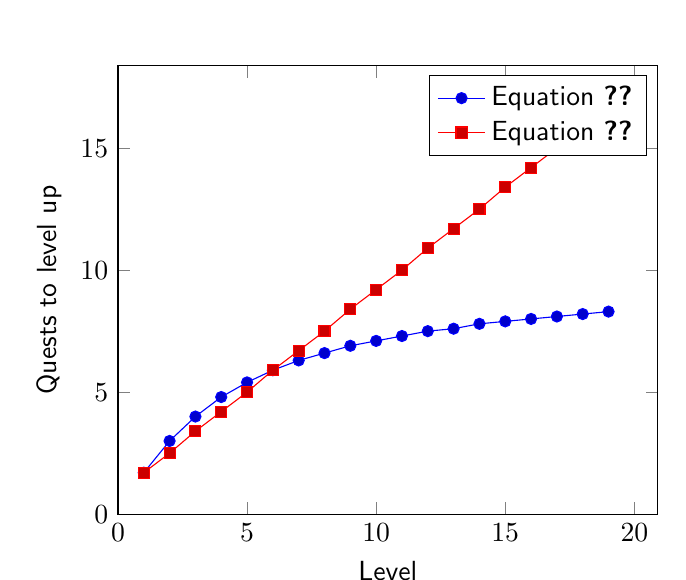
\begin{tikzpicture}
	\begin{axis}[
		xlabel=Level,
		ylabel=Quests to level up,
		xmin=0,
		ymin=0,
	]
		\addplot coordinates {
			(1, 1.7)
			(2, 3)
			(3, 4)
			(4, 4.8)
			(5, 5.4)
			(6, 5.9)
			(7, 6.3)
			(8, 6.6)
			(9, 6.9)
			(10,7.1)
			(11,7.3)
			(12,7.5)
			(13,7.6)
			(14,7.8)
			(15,7.9)
			(16,8)
			(17,8.1)
			(18,8.2)
			(19,8.3)
		};
		\addlegendentry{Equation \ref{eq:xpgainedtriangular}}
		\addplot coordinates{
			(1, 1.7)
			(2, 2.5)
			(3, 3.4)
			(4, 4.2)
			(5, 5)
			(6, 5.9)
			(7, 6.7)
			(8, 7.5)
			(9, 8.4)
			(10, 9.2)
			(11, 10)
			(12, 10.9)
			(13, 11.7)
			(14, 12.5)
			(15, 13.4)
			(16, 14.2)
			(17, 15)
			(18, 15.9)
			(19, 16.7)
		};
		\addlegendentry{Equation \ref{eq:xpgainedlinear}}
	\end{axis}
\end{tikzpicture}
\end{center}

\subsection{Gold Rewards}
\begin{equation} \label{eq:openloopreward}
	yk = ax_k + by_{k-1} + cy_{k-2}lc
\end{equation}


%500-1000 words
%!TEX root = ../main.tex
\chapter{Conclusion}

This is the conclusion part



Word count: 9983

%TC:ignore

%\nocite{*} %Take this out if you don't want it to show all the references and only the ones you've referenced 
%30-50 references traditionally.
\bibliography{references}

%!TEX root = ../main.tex
\begin{appendices}

%!TEX root = ../chapters/appendix.tex
\chapter{MoSCoW}

\subsubsection{Must have}
\begin{itemize}
	\item Parent control app
	\item Task management
	\item RPG elements
	\item Quest rewards
	\item Gold rewards
\end{itemize}

\subsubsection{Should have}
\begin{itemize}
	\item Full REST backend
	\item Preset/Trending quests
	\item Friends list
\end{itemize}

\subsubsection{Could have}
\begin{itemize}
	\item Graph friend selection 
	\item Friend battles
	\item Web application
\end{itemize}

\subsubsection{Won't have}
\begin{itemize}
	\item Sound effects
	\item Full character graphics
	\item Leaderboards
\end{itemize}

\chapter{Sheldon Book Grading Structure}

%!TEX root = ../chapters/appendix.tex
\chapter{Notifications}
\label{appendix:pushnotifications}

\centering
\begin{tabular}{|c|c|}
	\hline
	\textbf{Event} & \textbf{Notifcation Text} \\
  	\hline
  	Quest Complete & ``You have completed a quest!'' \\
  	\hline
  	Quest Confirmed & ``A child you are monitoring has finished a task and requires approval'' \\
  	\hline
  	Quest Added & ``A new quest is available!'' \\
  	\hline
  	Level Up & ``You have levelled up!'' \\
  	\hline
  	Reward Added & ``New rewards are available in the store!'' \\
  	\hline 
  	Reward Purchased & ``A child you are monitoring has purchased a reward from the store'' \\
  	\hline
\end{tabular}

\end{appendices}

%TC:endignore

\end{document}